\documentclass[10pt]{beamer}
\usepackage{amsmath,amssymb,longtable,hhline}
\usepackage{mathrsfs}
\usepackage{xcolor}
\usepackage{listings}
\usepackage{hyperref}
\usepackage{multicol}
\usepackage{anyfontsize}
\usepackage{minted}

\usemintedstyle{tango}
\newcommand{\ltprgsize}{\fontsize{5}{5}\selectfont}
\setminted{fontsize=\ltprgsize,mathescape}

\definecolor{mygreen}{rgb}{0,0.6,0}
\definecolor{mygray}{rgb}{0.5,0.5,0.5}
\definecolor{mymauve}{rgb}{0.58,0,0.82}

\hypersetup{
    bookmarks=true,         % show bookmarks bar?
    unicode=true,           % non-Latin characters in Acrobat’s bookmarks
    pdftoolbar=false,        % show Acrobat’s toolbar?
    pdfmenubar=false,        % show Acrobat’s menu?
    pdffitwindow=false,     % window fit to page when opened
    pdfstartview={FitH},    % fits the width of the page to the window
    pdftitle={Компьютерная алгебра в задачах оптимизации},    % title
    pdfauthor={Evgeny Cherkashin, Seseg Badmatsyrenova},     % author
    pdfsubject={symbolic computations},   % subject of the document
    pdfnewwindow=true,      % links in new PDF window
    colorlinks=true,       % false: boxed links; true: colored links
    linkcolor=red,          % color of internal links (change box color with linkbordercolor)
    citecolor=green,        % color of links to bibliography
    filecolor=magenta,      % color of file links
    urlcolor=blue           % color of external links
}

\lstset{language=Python,
  basicstyle=\footnotesize\ttfamily,        % the size of the fonts that are used for the code
  breakatwhitespace=false,         % sets if automatic breaks should only happen at whitespace
  breaklines=true,                 % sets automatic line breaking
  captionpos=b,                    % sets the caption-position to bottom
  commentstyle=\color{mygreen},    % comment style
  escapeinside={\%*}{*)},          % if you want to add LaTeX within your code
  extendedchars=true,              % lets you use non-ASCII characters; for 8-bits encodings only, does not work with UTF-8
%  frame=single,                    % adds a frame around the code
  keepspaces=true,                 % keeps spaces in text, useful for keeping indentation of code (possibly needs columns=flexible)
  keywordstyle=\color{blue},       % keyword style
%  numbers=left,                    % where to put the line-numbers; possible values are (none, left, right)
  numbersep=5pt,                   % how far the line-numbers are from the code
  numberstyle=\tiny\color{mygray}, % the style that is used for the line-numbers
  rulecolor=\color{black},         % if not set, the frame-color may be changed on line-breaks within not-black text (e.g. comments (green here))
  showspaces=false,                % show spaces everywhere adding particular underscores; it overrides 'showstringspaces'
  showstringspaces=false,          % underline spaces within strings only
  showtabs=false,                  % show tabs within strings adding particular underscores
  stepnumber=2,                    % the step between two line-numbers. If it's 1, each line will be numbered
  stringstyle=\color{mymauve},     % string literal style
  tabsize=2,                       % sets default tabsize to 2 spaces
%  title=\lstname                   % show the filename of files included with \lstinputlisting; also try caption instead of
}
\usepackage{pifont}

\usetheme{Warsaw}
\usecolortheme{crane}
%\useinnertheme{rectangles}
\setbeamertemplate{itemize item}{\scriptsize\hbox{\donotcoloroutermaths\ding{113}}}
\setbeamertemplate{itemize subitem}{\tiny\raise1.5pt\hbox{\donotcoloroutermaths$\blacktriangleright$}}
\setbeamertemplate{itemize subsubitem}{\tiny\raise1.5pt\hbox{\donotcoloroutermaths$\blacktriangleright$}}
\setbeamertemplate{enumerate item}{\insertenumlabel.}
\setbeamertemplate{enumerate subitem}{\insertenumlabel.\insertsubenumlabel}
\setbeamertemplate{enumerate subsubitem}{\insertenumlabel.\insertsubenumlabel.\insertsubsubenumlabel}
\setbeamertemplate{enumerate mini template}{\insertenumlabel}

\beamertemplatenavigationsymbolsempty

\usepackage{iftex,ifxetex}
\ifPDFTeX
  \usepackage[utf8]{inputenc}
  \usepackage[T1]{fontenc}
  \usepackage[russian]{babel}
  \usepackage{lmodern}
  \usefonttheme{serif}
\else
  \ifluatex
    \usepackage{unicode-math}
    \defaultfontfeatures{Ligatures=TeX,Numbers=OldStyle}
    \setmathfont{Latin Modern Math}
    \setsansfont{Linux Biolinum O}
    \setmonofont{Fira Mono}
    \usefonttheme{professionalfonts}
    % \setmathfont[
    %     Ligatures=TeX,
    %     Scale=MatchLowercase,
    %     math-style=upright,
    %     vargreek-shape=unicode
    %     ]{euler.otf}
  \fi
\fi

%\useoutertheme{split}
%\useinnertheme{rounded}
\setbeamertemplate{background canvas}[vertical shading][bottom=white!80!cyan!20,top=cyan!10]
%\setbeamertemplate{sidebar canvas left}[horizontal shading][left=white!40!black,right=black]

\graphicspath{{pics/}}

\providecommand{\email}[1]{\texttt{#1}}

% --------------------------

\begin{document}
\title[Model Driven Architecture using LOD]{Model Driven Architecture Implementation using Linked Data}
\author[E.~Cherkashin, A.~Kopaygorodsky, L.~Kazi, A.~Shigarov, V.~Paramonov]{\bfseries%
  Evgeny Cherkashin, Alexey Kopaygorodsky, Ljubica Kazi, Alexey Shigarov, Vyacheslav Paramonov}
\institute[ISDCT SB RAS, ESI SB RAS, ISC SB RAS, University of Novi Sad, Technical faculty "Mihajlo Pupin",
National Research Irkutsk State Technical University]{\normalsize ISDCT SB RAS, ESI SB RAS, ISC SB RAS, National Research Irkutsk State Technical University, Irkutsk,Russia,\\
  University of Novi Sad, Technical faculty "Mihajlo Pupin", Zrenjanin, Serbia\\[1em]
\email{\href{mailto:eugeneai@icc.ru}{eugeneai@icc.ru},\href{mailto:digger@istu.edu}{digger@istu.edu}}%
}
\date[2018]{{}\\
The 24${}^\text{th}$ International Conference on Information\\ and Software Technologies (ICIST 2018)\\
October 4${}^\text{th}$ -- 6${}^\text{th}$, 2018\\
Vilnius, Lithuania
}
%\date{\today}
\maketitle

\begin{frame}
  \frametitle{Model Driven Architecture and Linked Open Data}
  \begin{center}
    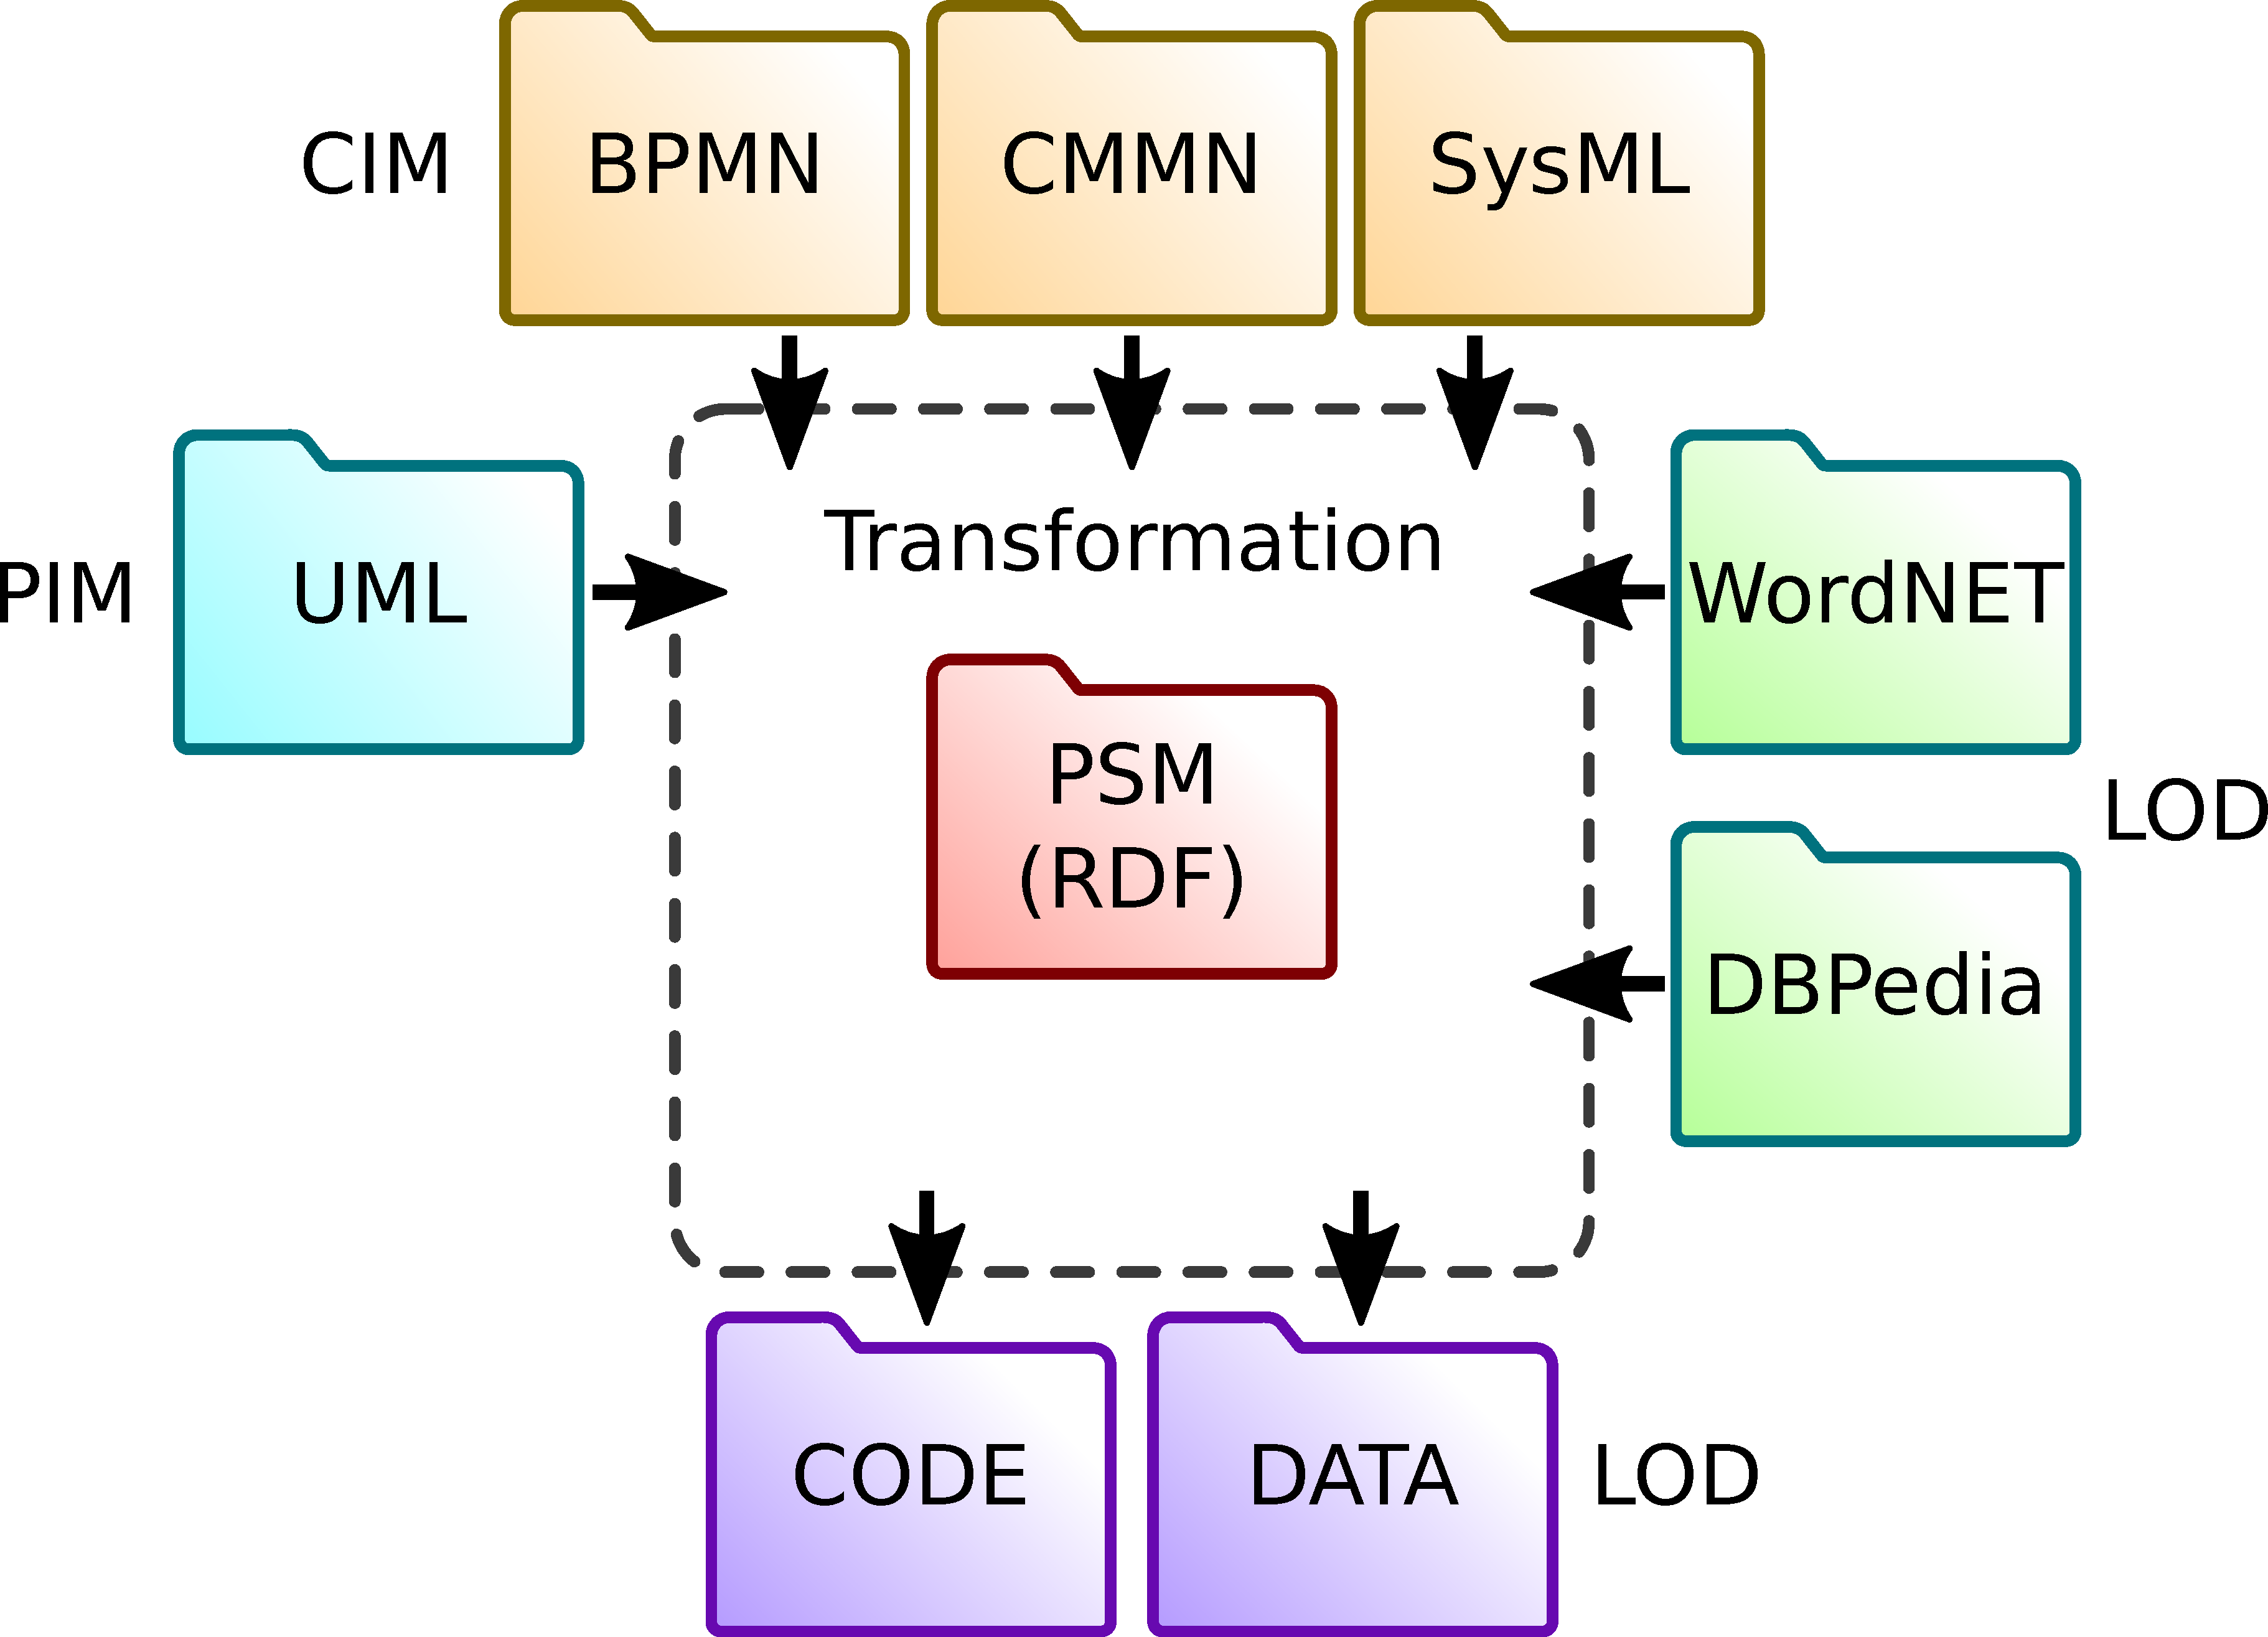
\includegraphics[width=0.9\linewidth]{mda-overview.pdf}
  \end{center}
\end{frame}

% ----------------------------------------------------------------
% \begin{frame}{Цели внедрения СМК ISO9001}
%   Соответствие медицинской организации стандарту ISO9001 -- демонстраци ее приверженности к высокой степени качества управления бизнес-процессами. В медицине только 4\% проблем созданы из-за ошибок персонала, 96\% из-за плохого управления.
%   \begin{block}{Сертификация соответствия стандарту дает}
%     \begin{itemize}
%     \item формальное признание качества обслуживания в России и за рубежом;
%     \item лучшие позиции в тендерах;
%     \item лучшие позиции среди конкурентов;
%     \item предпочтения со стороны иностранцев, работающих в России, для сотрудничества на международном уровне;
%     \item нахождение в <<клубе>> сотрудничающих учреждений и наличие <<преференций>>;
%     \item формальное соответствие отраслевым стандартам качества;
%     \item проведение этапа анализа учреждения, что приводит к лучшему пониманию целей, задач и процессов.
%     \end{itemize}
%   \end{block}
% \end{frame}
% \begin{frame}
%   \frametitle{СМК бизнес-процессов}
%   \begin{figure}[htb]
%     \centering
%     %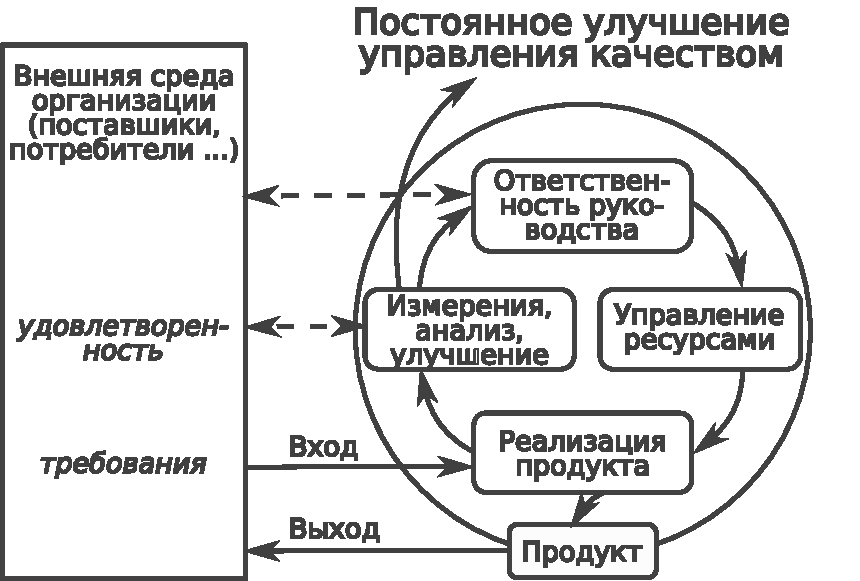
\includegraphics[width=0.9\linewidth]{iso9001-ru.pdf}
%     % \caption{A general view on the ISO 9001:2015}
%     \label{fig:iso9001}
%   \end{figure}
% \end{frame}
% \begin{frame}
%   \frametitle{Базис принятия решений}
%   Развитие предприятия основывается на \emph{решениях}, принимаемых на базе \emph{фактического материала}, который формируется в результате
%   \begin{itemize}
%   \item анализа \emph{ожиданий контрагентов}: \emph{потребностей клиента} и \emph{критериев качества} требуемого продукта;
%   \item определения \emph{элементарных целей} (unities of purpose);
%   \item поиска возможных направлений развития предприятия с учетом \emph{вовлеченности персонала}, т.е. личных интересов и целей;
%   \item моделирования производства или предоставляемой услуги как \emph{системы процессов}, что позволяет проводить \emph{локальные улучшения};
%   \item \emph{измерений} количественных и качественных параметров продукта и процессов.
%   \end{itemize}
% \end{frame}
\begin{frame}
  \frametitle{Goals}
  \textbf{Целью} исследования является создание методики разработки информационных систем поддержки СМК бизнес-процессов в медицинском учреждении (ГБУЗ <<Областной онкологический диспансер>>). Решаются задачи
  \begin{enumerate}
  \item Представления модели бизнес-процессов (БП) при помощи SysML, CMMN и BPMN2.0. \label{p1}
  \item Создание архитектуры средств MDA для трансформации CIM п.~\ref{p1} в PIM.
  \item Разработка средств трансформации PIM в PSM и далее в исходный код информационных систем (ИС) \emph{конструктивной} поддержки СМК.
  \item Бесшовная интеграция ИС с существующим программным обеспечением (ИС, ЛИС и т.д.)
  \end{enumerate}
\end{frame}
% \begin{frame}
%   \frametitle{Исходные данные (As Is)}
%   \begin{columns}[t]
%     \begin{column}{0.5\textwidth}
%     %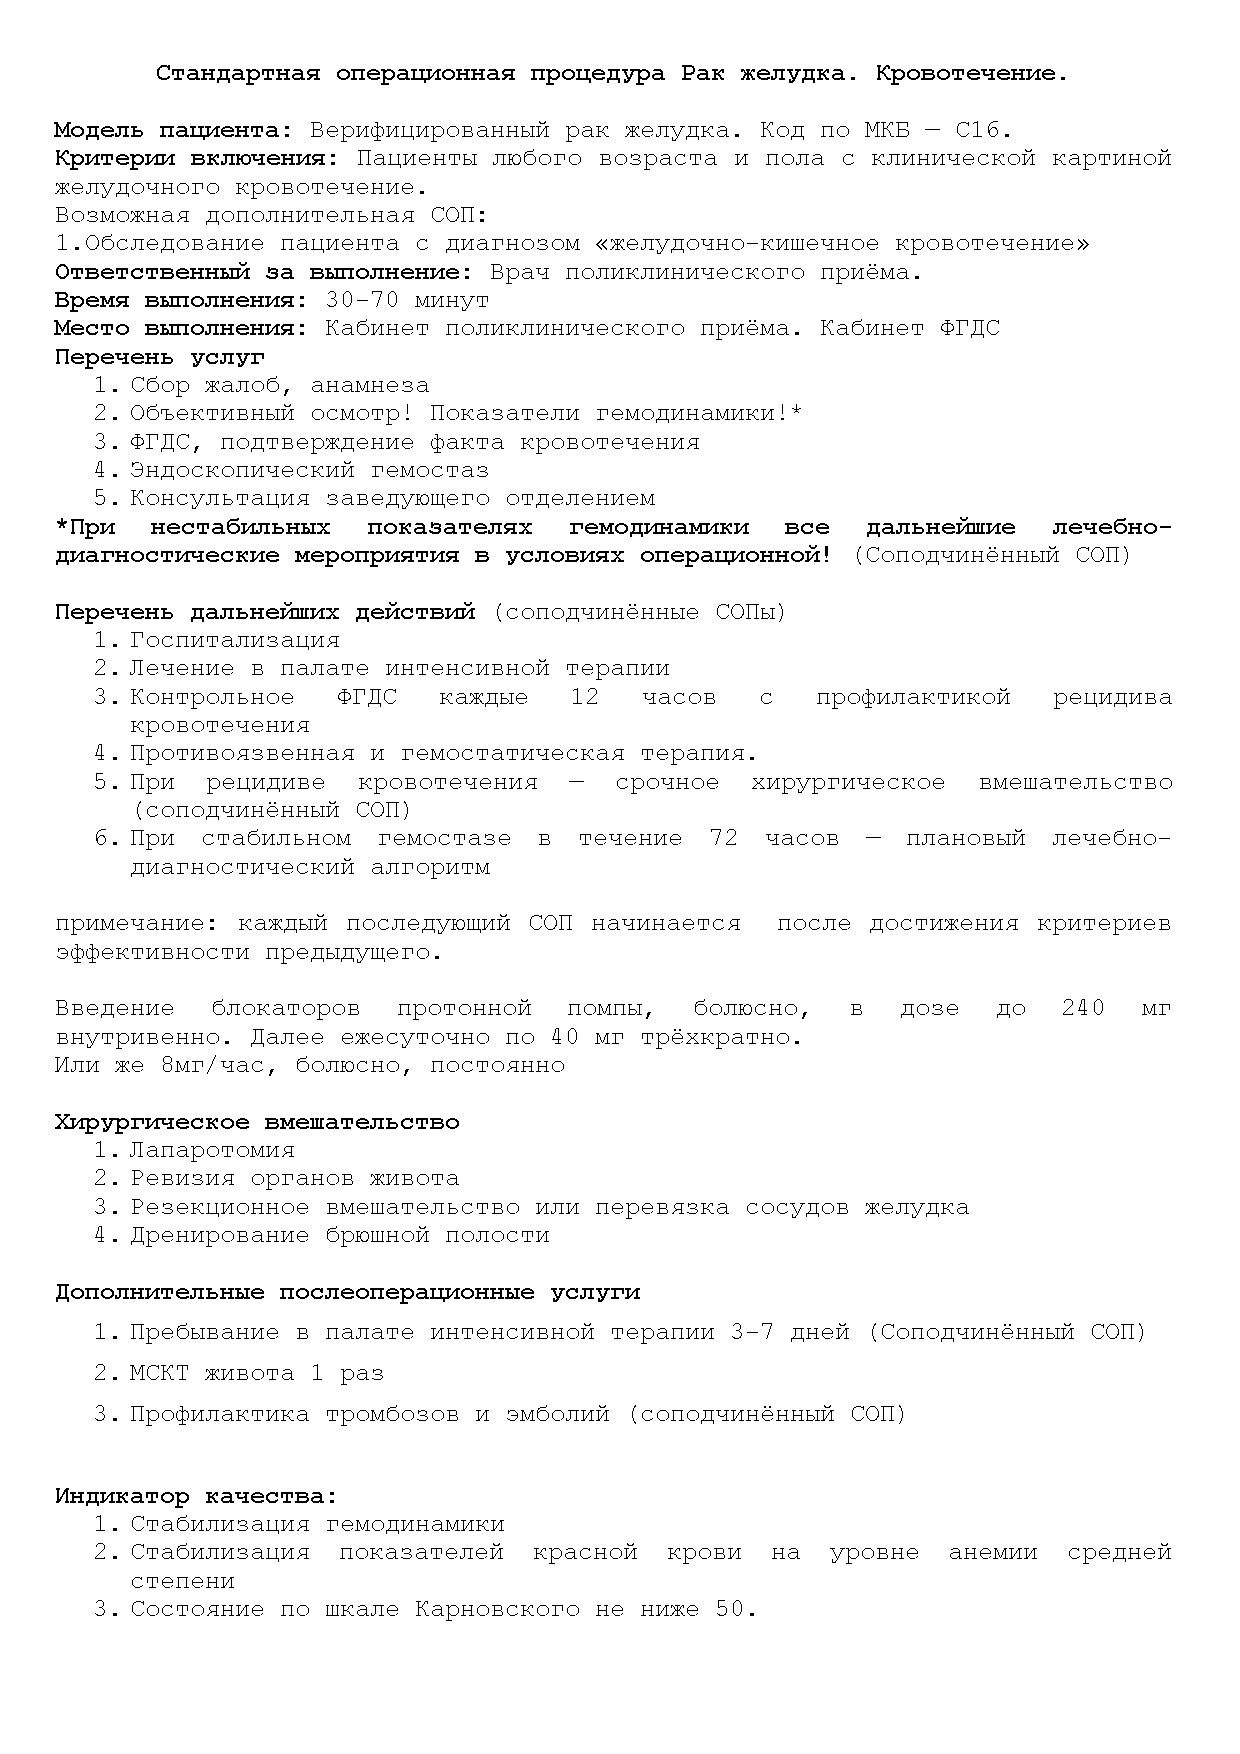
\includegraphics[width=1\linewidth]{sop-ex-1.pdf}
%     \end{column}
%     \begin{column}{0.5\textwidth}
%     %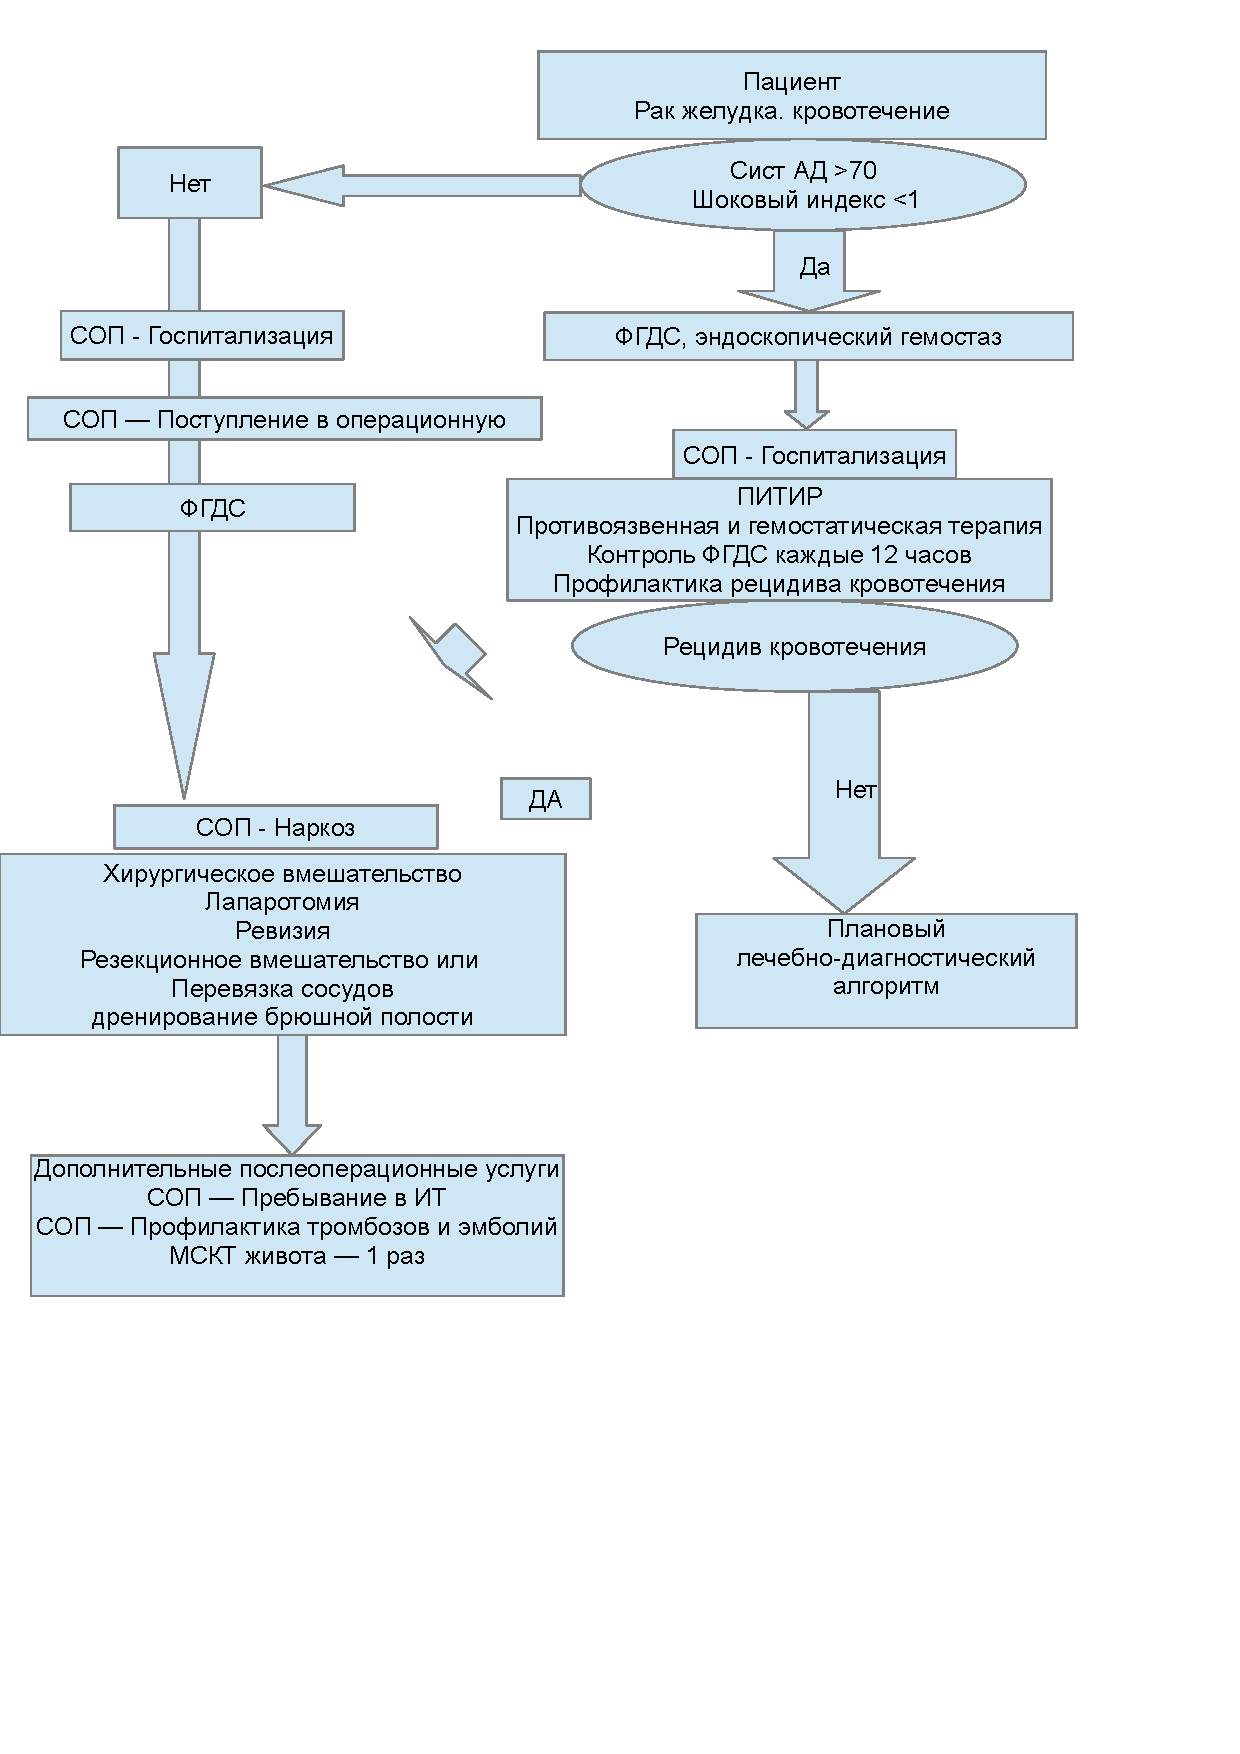
\includegraphics[width=1\linewidth]{sop-ex-2.pdf}
%     \end{column}
%   \end{columns}
% \end{frame}
% \begin{frame}
%   \frametitle{Диаграммы SysML }
%   \centering
%     %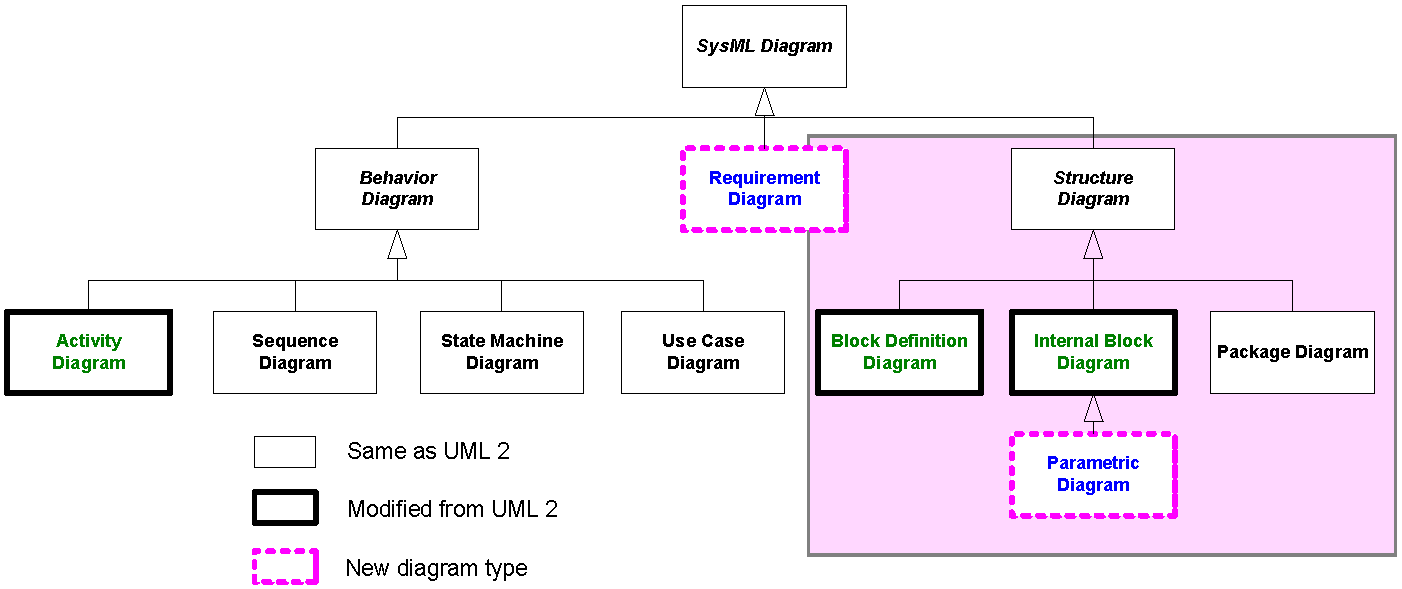
\includegraphics[width=1\linewidth]{diagrams.pdf}
% \end{frame}
% \begin{frame}
%   \frametitle{Диаграмма требований (Requirements Diagram)}
%   \centering
%     %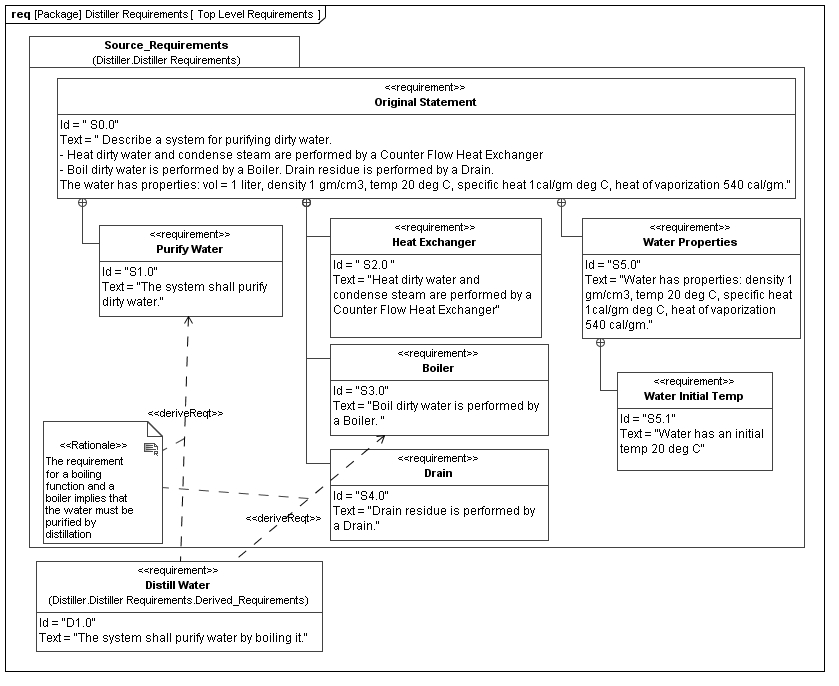
\includegraphics[width=0.9\linewidth]{req-ex.png}
% \end{frame}
% \begin{frame}
%   \frametitle{Диаграмма параметров (Parametric Diagram)}
%   \centering
%     %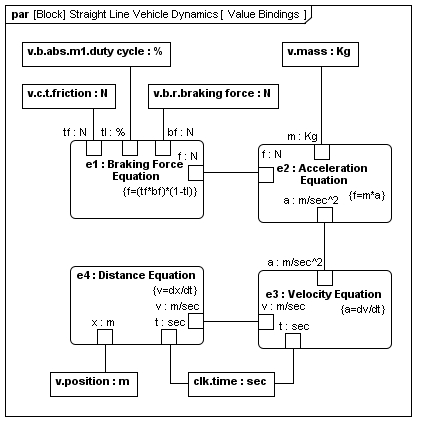
\includegraphics[width=0.7\linewidth]{par-ex.png}
% \end{frame}
% \begin{frame}
%   \frametitle{Диаграмма BPMN2.0}
%   BPMN -- Business process modeling notation
%   \centering
%     %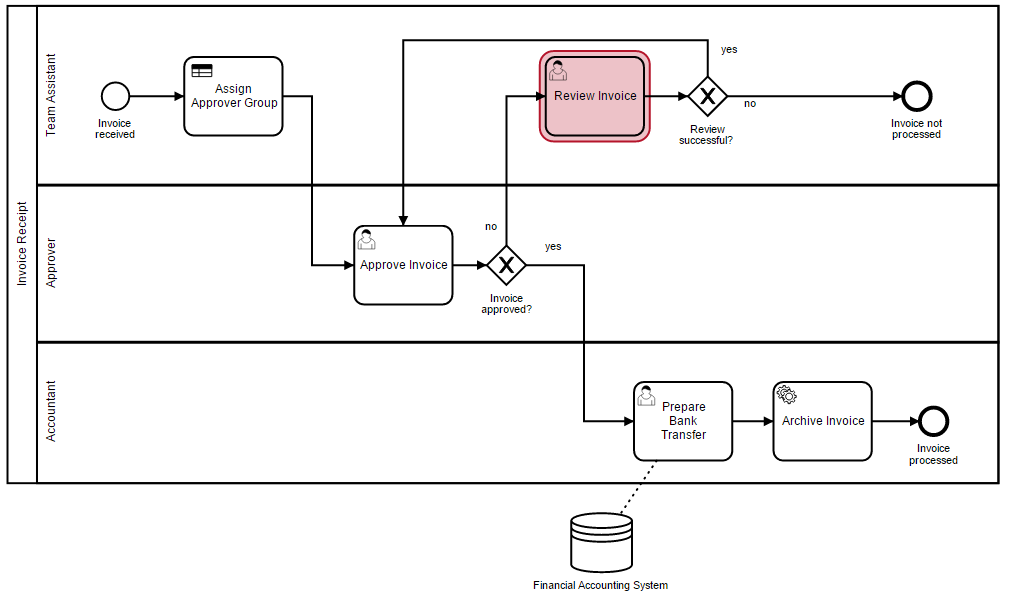
\includegraphics[width=1\linewidth]{bpmn.png}
% \end{frame}
% \begin{frame}
%   \frametitle{Диаграмма CMMN1.1}
%   CMMN -- Case management model and notation
%   \centering
%     %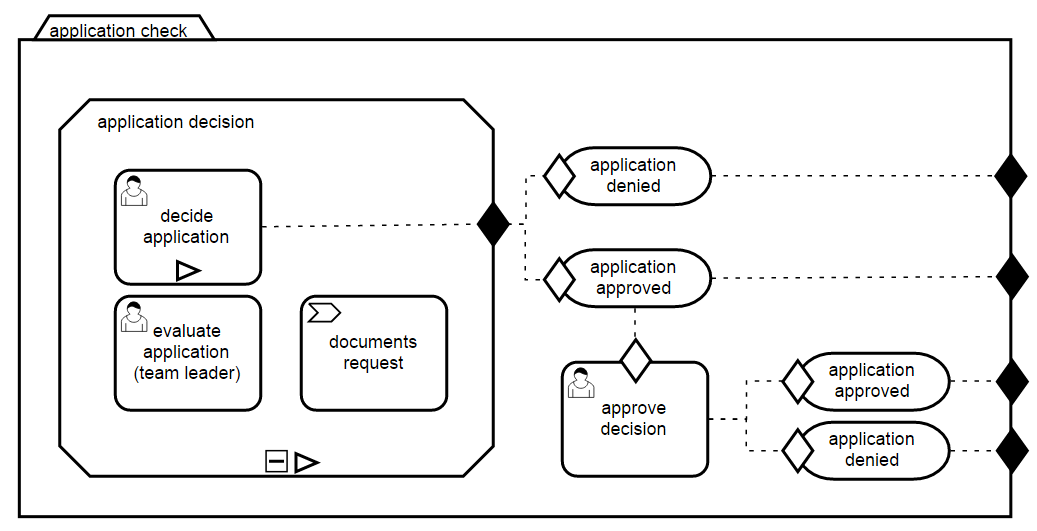
\includegraphics[width=1\linewidth]{cmmn.png}
% \end{frame}

\begin{frame}
  \frametitle{MDA component architecture}
  \centering
  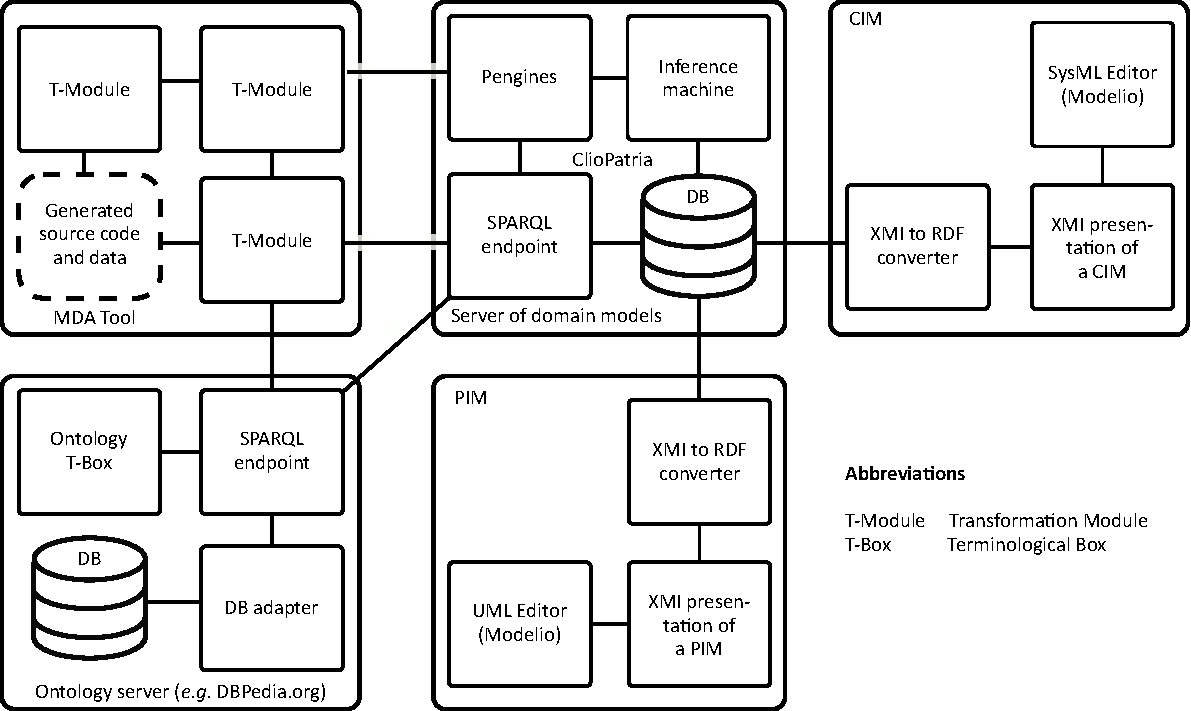
\includegraphics[width=1\linewidth]{architecture-mda-lod-ext.pdf}
\end{frame}

\begin{frame}
  \frametitle{Architecture of transformation modules}
  \centering
  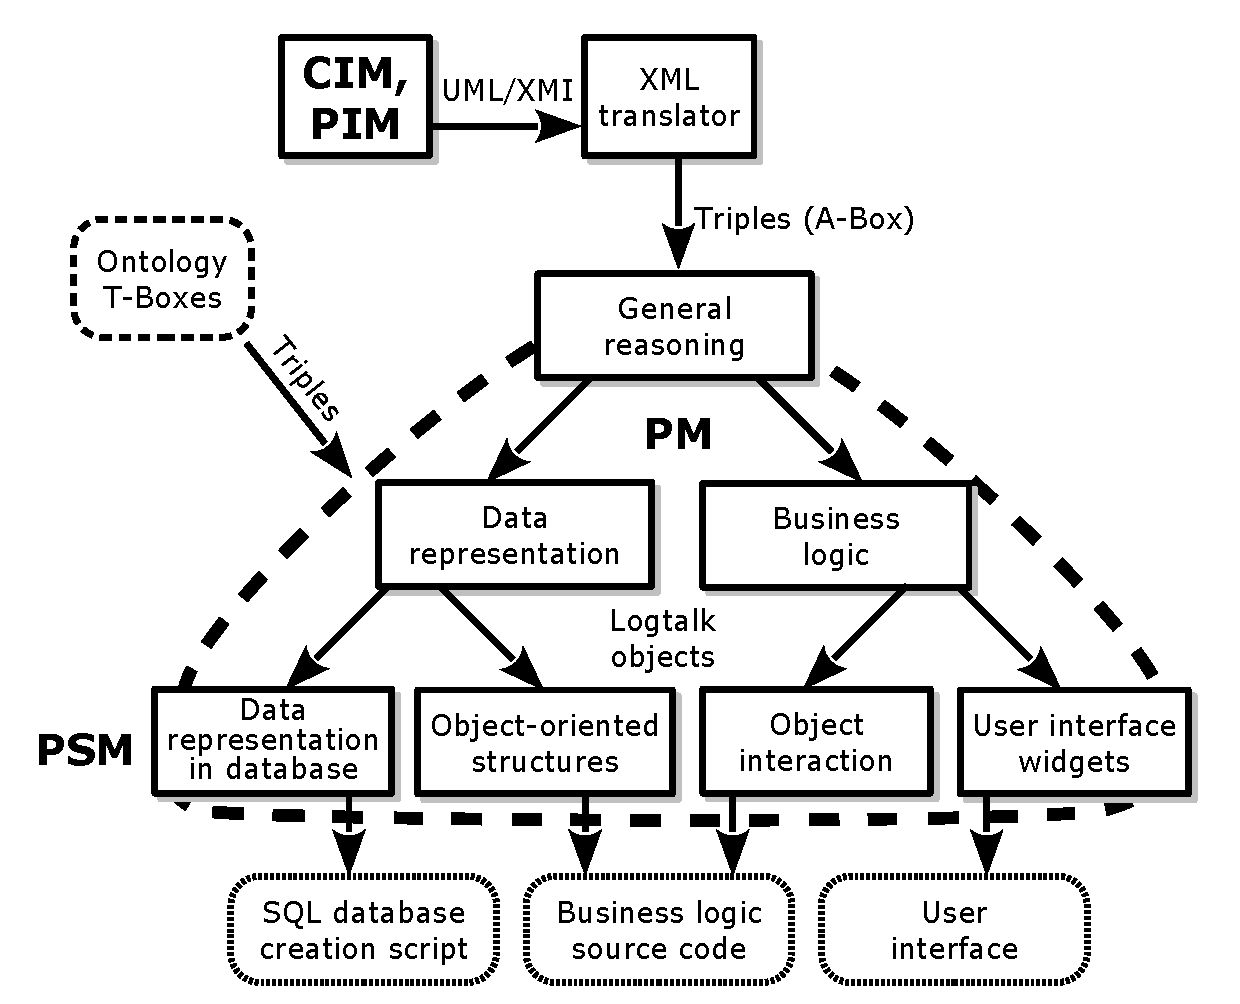
\includegraphics[width=0.9\linewidth]{architect_tree_pres-en-wo-OCL.pdf}
\end{frame}

\begin{frame}[fragile]
  \frametitle{PSM: Class structure inference}

%\begin{multicols}{2}
\begin{minted}{logtalk}
:- object(direct(_Package,_LocalProf,_CodeProf)).    % Параметризованный объект для синтеза
:- public([tr/4,tr/3]).                              % определения класса
:- protected([package/1, profiles/2, profile/1]).
package(Package):- parameter(1, Package).            % Интерфейс к параметрам объекта
profile(Profile):- parameter(2, Profile).
profile(Profile):- parameter(3, Profile).
profiles(L):-
    findall(Profile, ::profile(Profile), L).
tr(class, Class, ClassID):- ::package(Package),      % Синтез класса (первый параметр метода)
    query(Package)::class(Name, ClassID),            % Запрос к структуре пакета XMI
    create_object(Class,                             % Создание экземпляра объекта <<Класс>>
        [instantiates(class)],[],[]),
    create_object(Attributes,                        % Создание объекта <<Атрибуты>>
        [instantiates(params)],[],[]),
    create_object(Methods,                           % ...<<Методы>>.
        [instantiates(methodlist)],[],[]),
    Class::name(Name),                               % Задать имя классу.
    forall(                                          % Странсформировать атрибуты класса,
        ::tr(attribute,Attribute,ClassID,_AttrID),   % добавляя каждый в общий список.
        Attributes::append(Attribute) ),
    forall(                                          % ...методы...
        ::tr(method, Method, ClassID, _MethodID),
        Methods::append(Method) ),
    Class::attributes(Attributes),                   % Задать классу атрибуты.
    Class::methods(Methods).                         % ...методы.
tr(attribute, Attribute, ClassID, AttributeID):-     % Трансформация атрибута
    ::package(Package),
    query(Package)::attribute(Name,ClassID,AttrID),
    create_object(Attribute,
        [instantiates(param)],[],[]),
    Attribute::name(Name).                           % Задать имя атрибуту.
tr(method, Method, ClassID, MethodID):-              % Трансляция метода
    ::package(Package),
    query(Package)::method(Name,ClassID,MethodID),
    create_object(Method,
    [instantiates(method)],[],[]),
    Method::name(Name).                              % Имя метода
:- end_object.                                       % Граница объекта
\end{minted}
%\end{multicols}
\end{frame}

\begin{frame}[fragile]
  \frametitle{Implementation of \texttt{Query} object}
\begin{minted}[fontsize=\footnotesize{}]{logtalk}
:- object(query(_XMI)).
:- protected(xmi/1).
:- public([class/2, attribute/3, method/3]).
xmi(XMI) :- parameter(1, XMI).
class(Name, ID):-               % Распознавание класса в RDF
    ::xmi(XMI),
    XMI::rdf(ID,rdf:type,uml,'Class'),
    XMI::rdf(ID,rdfs:label, literal(Name)).
attribute(Name, ClassID, ID):-  % ...атрибута...
    ::xmi(XMI),
    XMI::graph(G),
    XMI::rdf(ClassID, G:ownedAttribute, ID),
    % XMI::rdf(ID, rdf:type, uml,'Property'),
    XMI::rdf(ID, rdfs:label, literal(Name)).
method(Name, ClassID, ID):-     % ...метода...
    ::xmi(XMI),
    XMI::graph(G),
    XMI::rdf(ClassID, G:ownedOperation, ID),
    XMI::rdf(ID, rdfs:label, literal(Name)).
:- end_object.
\end{minted}
\end{frame}

\begin{frame}[fragile]
  \frametitle{Code Bloock}
  Идея реализации взята из библиотеки \verb|llvmlib|.
\begin{minted}{logtalk}
:- object(code_block, specializes(root)).
:- public([append/1, prepend/1, clear/0,      % Внешний интерфейс объекта
   render/1, render_to/1, remove/1, item/1,
   items/1 ]).
:- dynamic([item_/1]).                        % Элементы кодового блока
:- private([item_/1]).
:- protected([renderitem/2, render_to/2]).    % Методы, специализируемые при наследовании

item(Item)   :- ::item_(Item).
items(Items) :- bagof(I, ::item(I), Items).
append(Item) :- ::assertz(item_(Item)).       % Добавить элемент в конец
prepend(Item):- ::asserta(item_(Item)).       % ...в начало
remove(Item) :- ::retract(item_(Item)).       % Удалить элемент
clear        :- ::retractall(item_(_)).       % Очистить блок кода.
render(_)    :- writef::writef("ERROR: \      % Преобразовать блок в исходный код
Implement render/1 by a subclass!\n"), fail.

render_to(Stream):- ::render(List),
    ::render_to(List, Stream).
render_to(List, Stream):-
    lists::is_list(List),!,
    forall(lists::member(X,List),
       ::render_to(X, Stream)).
render_to(X,_) :- write(X),nl.
renderitem(Object, String):-                  % Способ преобразования элемента-объекта
    current_object(Object), !,                % по умолчанию (попросить его самого это сделать)
    Object::render(String).
renderitem(literal(Item), String):-!,         % Преобразование литерала (строка, число,...)
    atom_string(Item, String).
renderitem(Item, String):-                    % ...строки.
    root::iswritef(String, '%q', [Item]).
:- end_object.
\end{minted}
\end{frame}

\begin{frame}[fragile]
  \frametitle{Generation of a Python Class}
  Класс-генератор -- это специализация кодового блока.  Элементами блока являются другие блоки: список наследуемых классов, список атрибутов и список методов.

  Чтобы сгенерировать исходный код класса, сначала надо сформировать кодовые блоки, и затем запустить \verb|render/1|. В переменную \verb|Result| помещается список строк кода.
\begin{multicols}{2}
\begin{minted}{logtalk}
:- object(class, specializes(code_block),
   imports([named])). % Категория поименованных сущностей
:- public([classlist/1, methods/1, attributes/1]).
classlist(ClassList):- % Список наследуемых классов
    ::prepend(classlist(ClassList)).
attributes(Attributes):- % Список атрибутов
    ::prepend(attributes(Attributes)).
methods(MethodList):-    % Список методов
    ::append(methods(MethodList)).

renderitem(Item, Result):- % по умолчанию
    ^^renderitem(Item, Result).
render(Result):-         % Генератор кода
    ^^render(Name),
    ( ::item(classlist(List)) ->
      List::render(ClassList),
      root::iswritef(Signature,'class %w(%w):',
        [Name, ClassList]);
      root::iswritef(Signature,'class %w:',
        [Name]) ),
    root::indent,        % добавить отступ
    ( ::item(attributes(Attributes))->
      Attributes::render(DefAttrList),
      root::iswritef(ConstructorDef,
        'def __init__(self, %w):',
        [DefAttrList]),
      root::indent,      % еще отступ
      Attributes::items(InstanceAttrs),
      findall(S, ( % инициализация атрибутов
         lists::member(Attr, InstanceAttrs),
         Attr::item(name(AttrName)),
         root::iswritef(S, "self.%w=%w",
           [AttrName, AttrName])
         ), AttrAssigns),
        root::unindent,
        AttrList=[ConstructorDef|AttrAssigns];
        root::iswritef(ConstructorDef,
          'def __init__(self): ', []),
        root::indent,
        root::iswritef(Pass,'pass', []),
        root::unindent,
        AttrList=[ConstructorDef, Pass] ),
    ( ::item(methods(Methods))-> % Если есть...
      Methods::render(MethodList);
      MethodList=[] ),
    lists::append(AttrList,MethodList,StringList),
    root::unindent, Result=[Signature|StringList].
:- end_object.
\end{minted}
\end{multicols}
\end{frame}

\begin{frame}[fragile]
  \frametitle{Logtalk Categories}
  Категория поименованных сущностей
\begin{minted}{logtalk}
:- category(named).
:- public([name/1, render/1]).
:- protected([renderitem/2]).
name(Name):- ::prepend(name(Name)).
renderitem(name(Name), String):-!, atom_string(Name, String).
render(String):-  % Как генерировать код
    ::item(name(Name)),
    ::renderitem(name(Name), String).
:-end_category.
\end{minted}
Категория поименованных сущностей, имеющих тип
\begin{minted}{logtalk}
:- category(namedtyped, extends(named)).
:- public([type/1,render/2, separator_option/2,list_separator/1]).
:- protected([renderitem/2]).
type(Type):- ::append(type(Type)).
renderitem(Item, String):-
    ^^renderitem(Item, String),!.
renderitem(type(Type),String):-!,
    ::list_separator(Separator),
    writef::swritef(String, '%w%w', [Separator, Type]).
render(Middle, String):-
    ^^render(SName),
    (   ::item(type(Type)) ->
        ::renderitem(type(Type), SType),
        string_concat(SName, Middle, _1),
        string_concat(_1, SType, String) ;
        SName = String  ).
render(String):-  ::render("", String).

list_separator(Separator):-
    ::separator_option(Name, Default),!, % Глобальные настройки
    root::option(Name, Separator, Default).
:- end_category.

\end{minted}
\end{frame}

% \begin{frame}
%   \frametitle{Общий план разработки ИС поддержки БП}
%   На начальном этапе применения разработанных технологий предполагается организовать развитие ИС в соответствии со следующими этапами:
%   \begin{enumerate}
%   \item Преобразование CIM в чек-листы, заполняемые медсестрами, что позволит контролировать готовность пациента к операции, манипуляции, анализам и т.п.;
%   \item Планирование лечения пациента после операции;
%   \item Организация системы взаимодействия с клиентами, например, планирование диспансеризации населения.
%   \end{enumerate}
% \end{frame}

\begin{frame}
  \frametitle{Applications}

\end{frame}

\begin{frame}
  \frametitle{Conclusion}
  Основная решаемая задача в исследовании -- изучить применимость SysML, BPMN и CMMN в качестве CIM при разработке информационных систем. Кроме того
  \begin{itemize}
  \item В рамках возможного реинжениринга БП ИООД создать платформу интеграции существующих ИС друг с другом и бизнес-процессами <<To Be>>.
  \item Создать инструментальные средства MDA для порождения каркасов информационных систем на основе сформированных моделей БП.
  \end{itemize}
\end{frame}

\end{document}

%%% Local Variables:
%%% mode: latex
%%% TeX-master: t
%%% End:
